% !TeX spellcheck = en_GB

\begin{figure}[h!]
    \centering
%%%%%% 20/12
    \begin{subfigure}[b]{0.49\textwidth}
        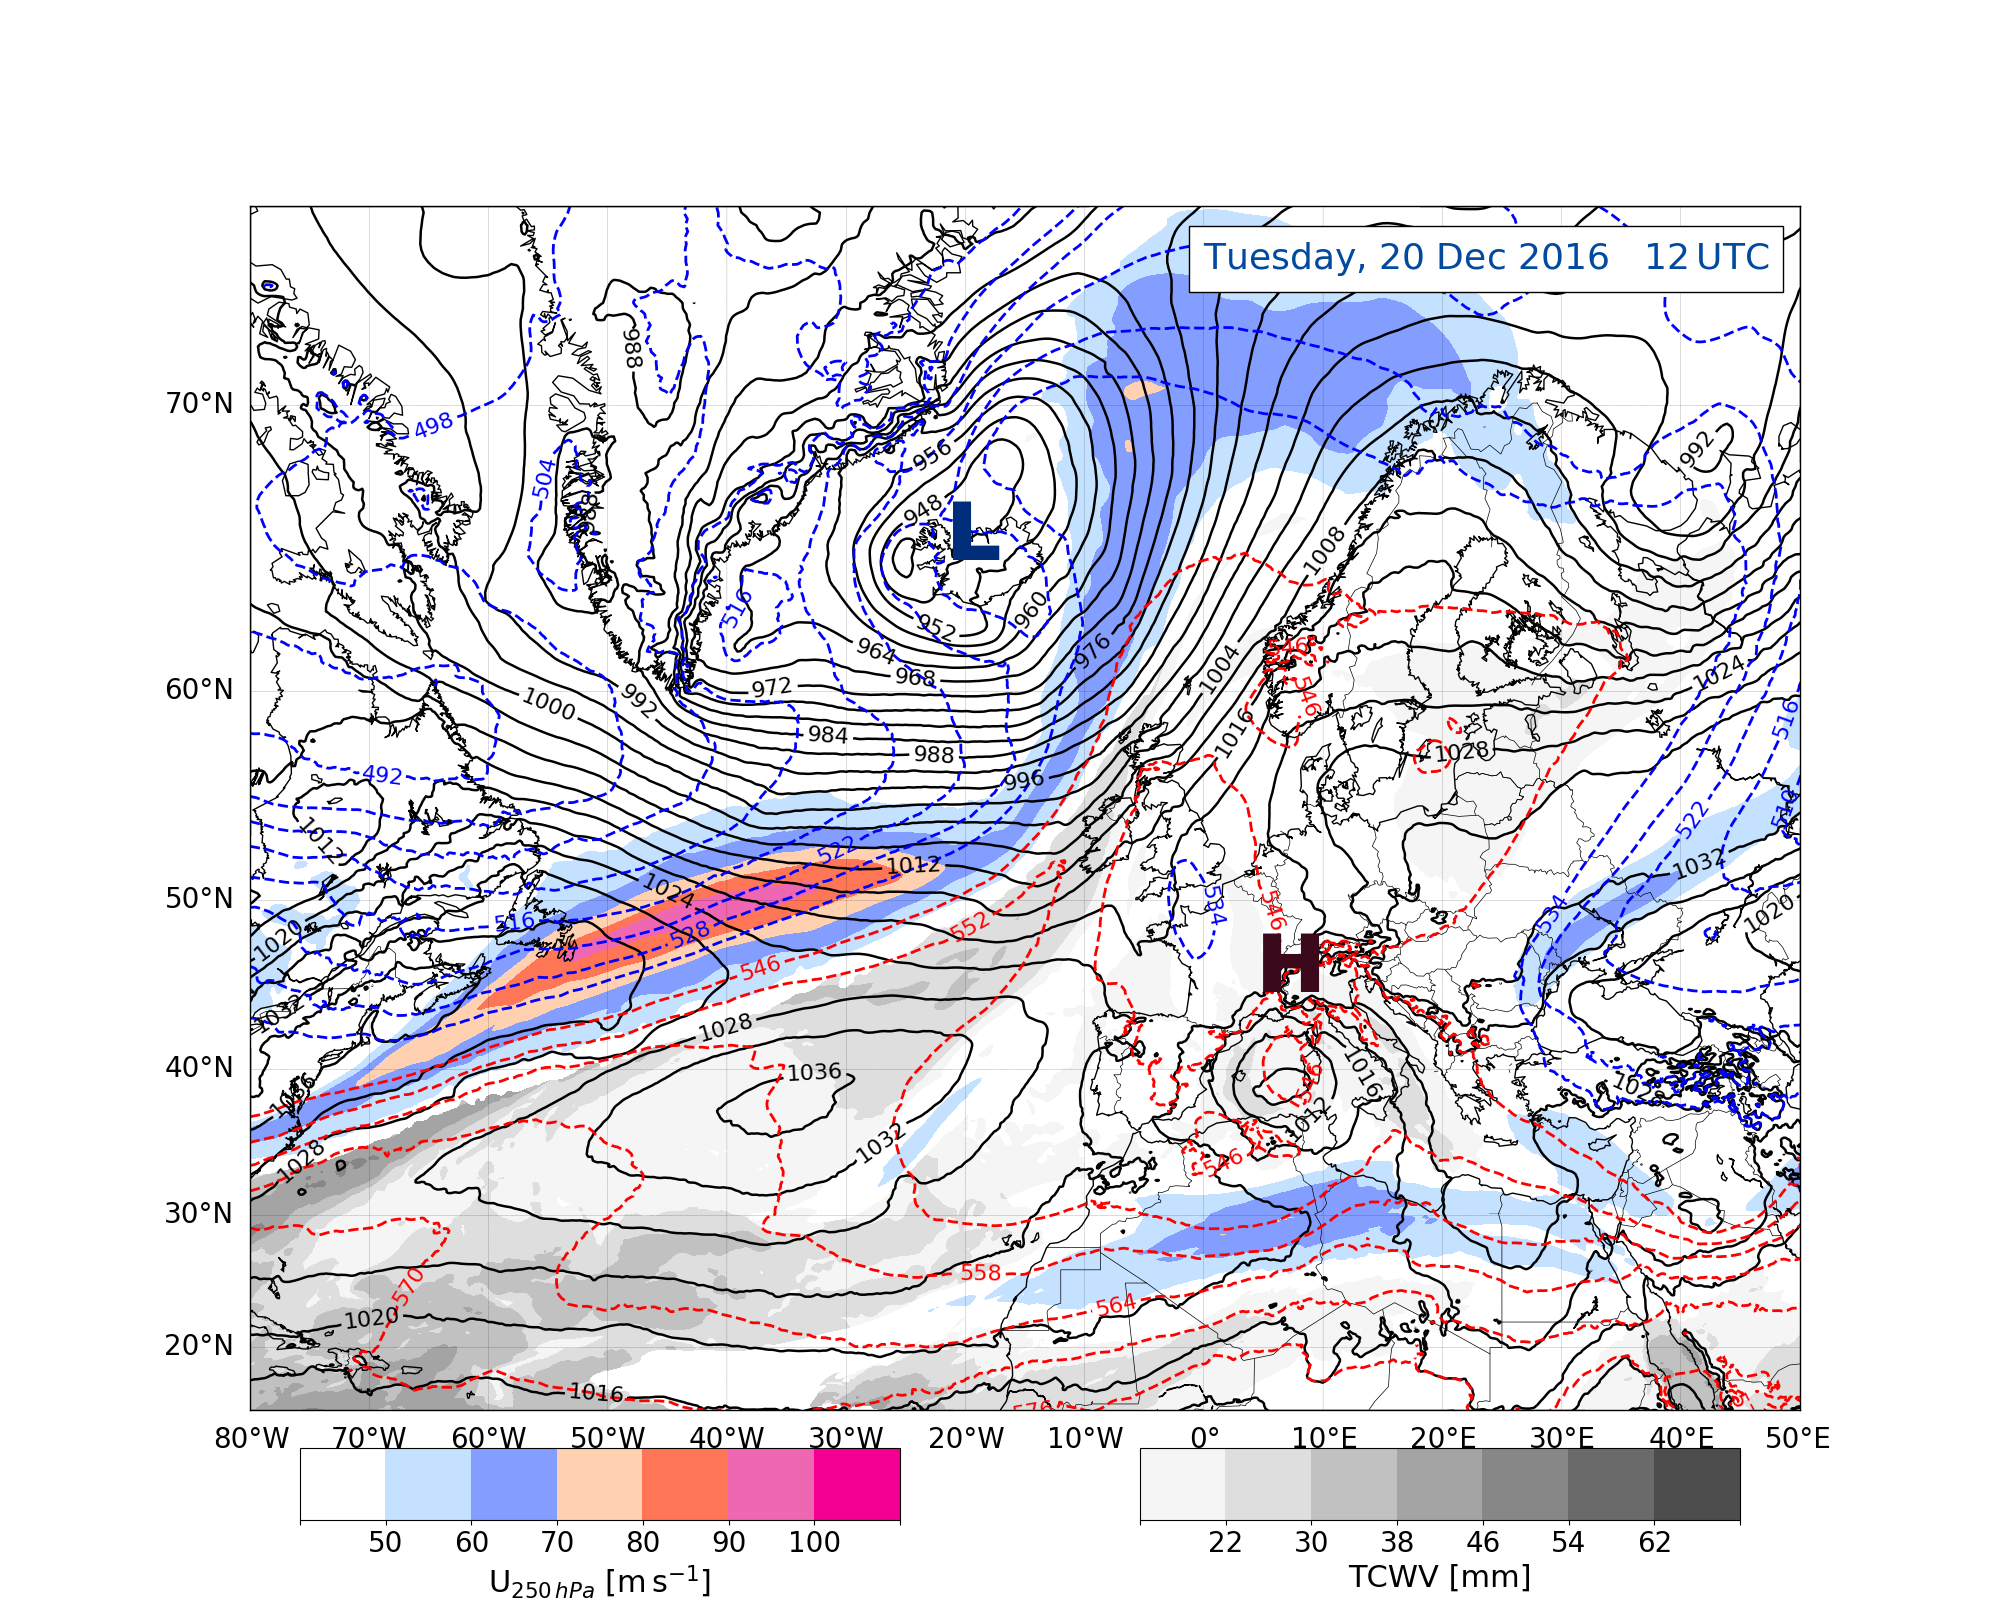
\includegraphics[trim={4.2cm 3.9cm 4.3cm 5.1cm},clip,
        width=\textwidth]{./fig_Geopot_Jet/20161220_12}
        \caption{}\label{fig:GP20}
        %\label{fig:DT2100}
    \end{subfigure}
%%%%%% 21/12
    \begin{subfigure}[b]{0.49\textwidth}
        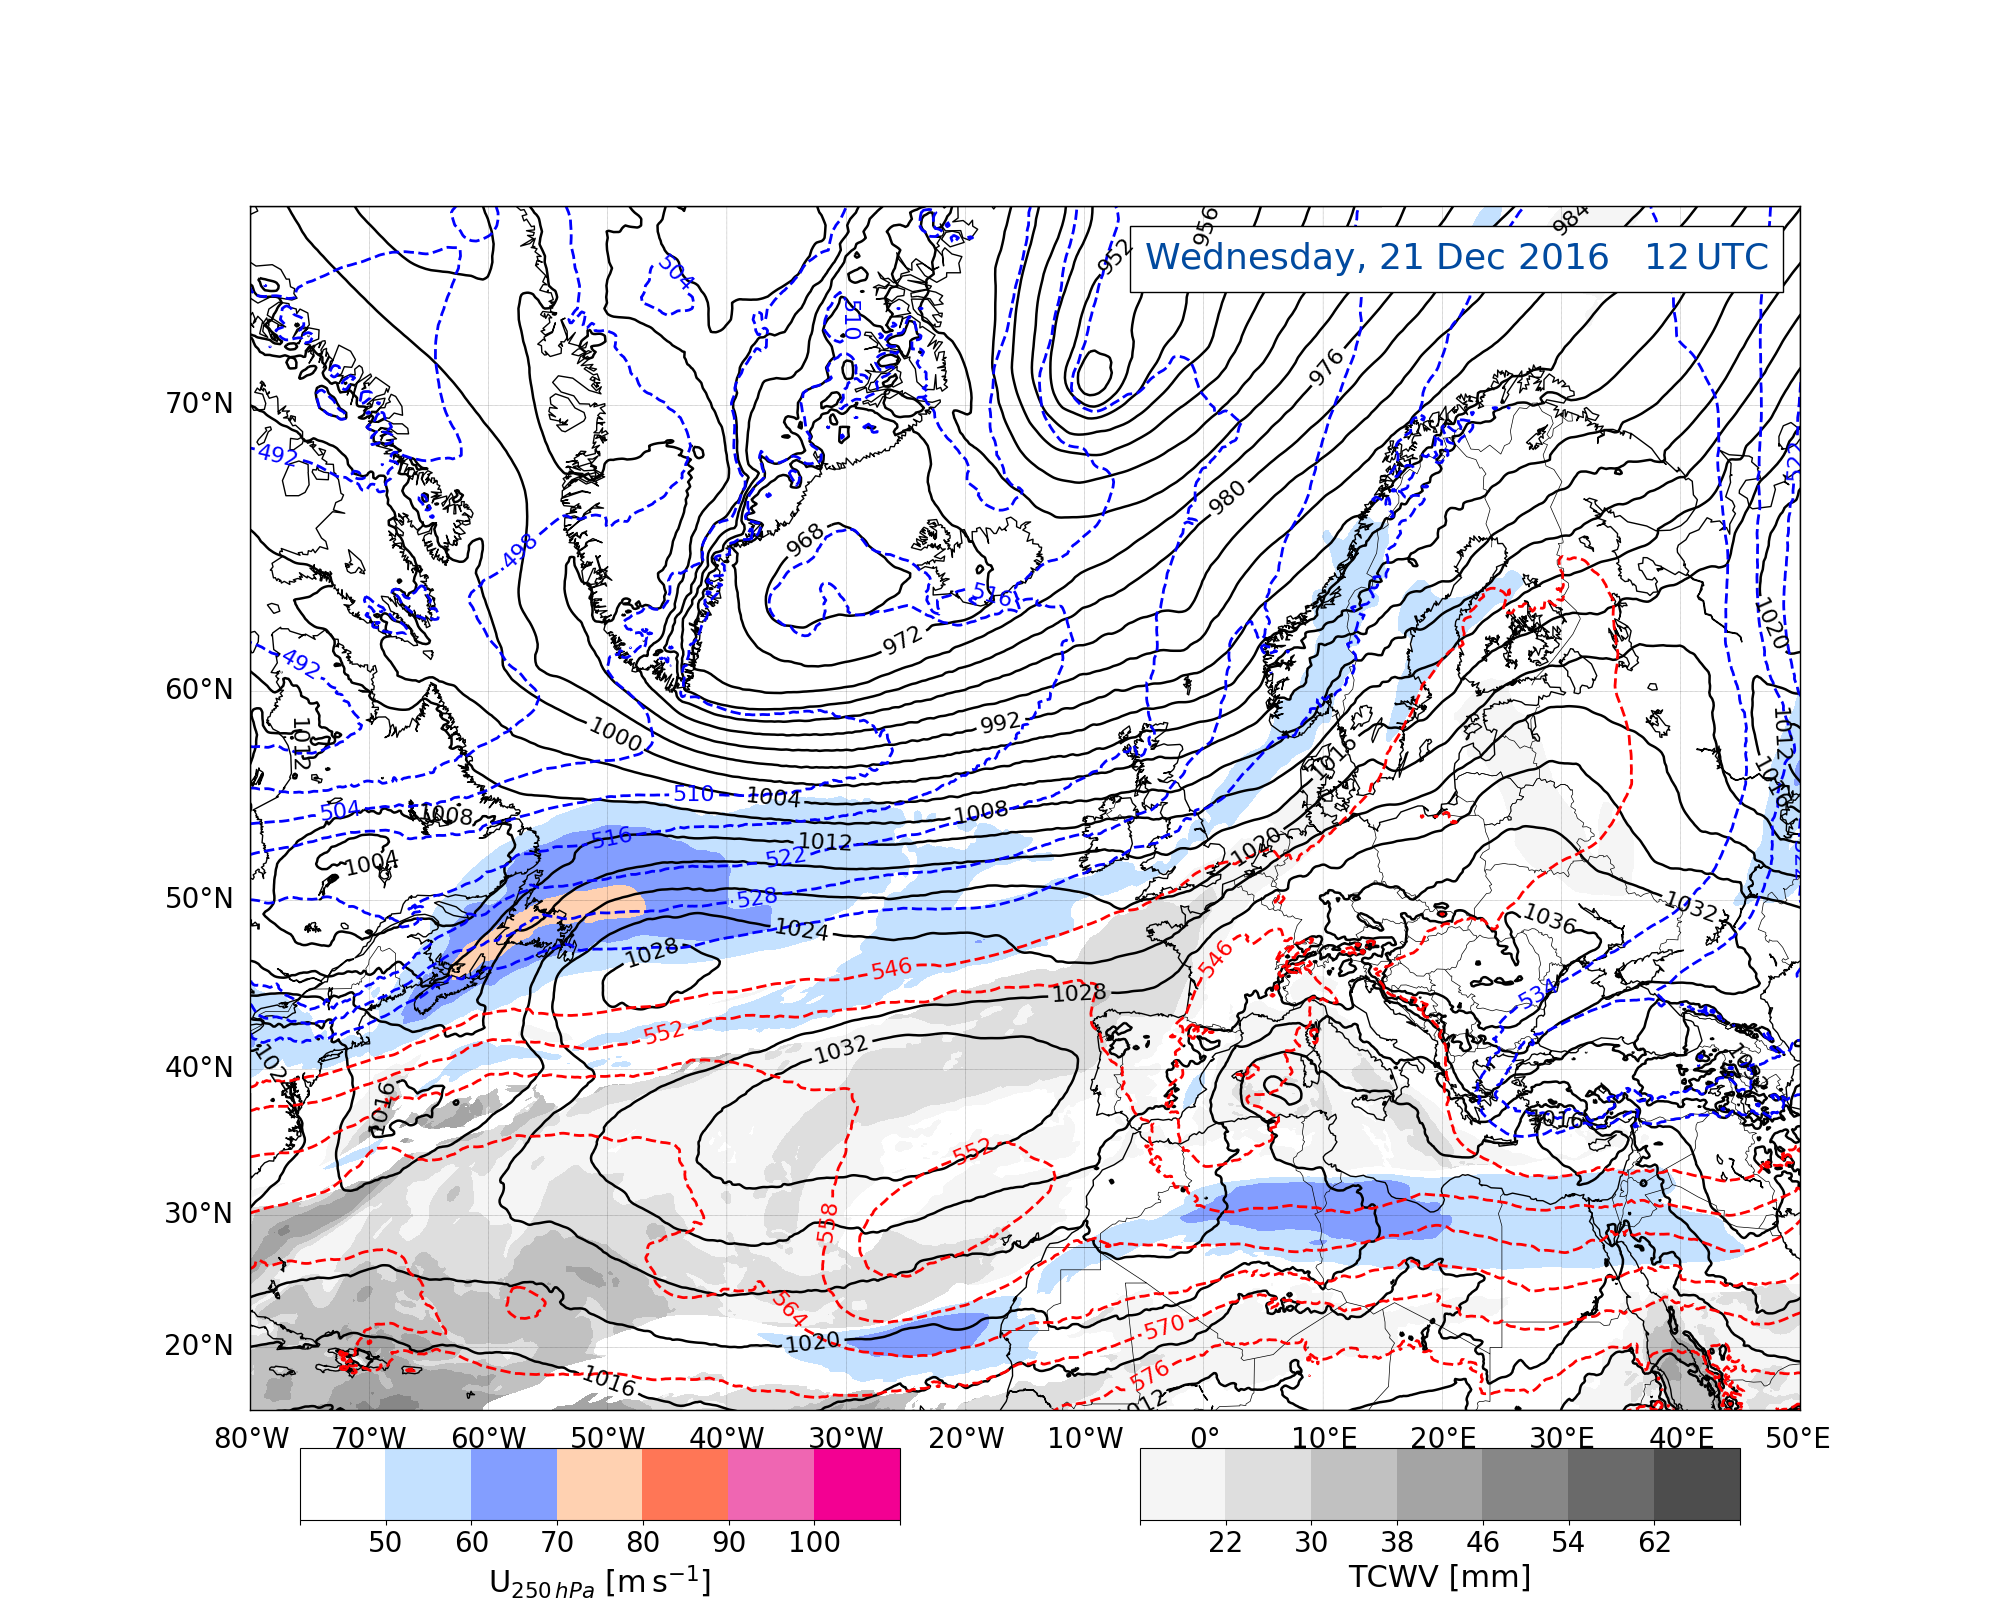
\includegraphics[trim={4.2cm 3.9cm 4.3cm 5.1cm},clip,
        width=\textwidth]{./fig_Geopot_Jet/20161221_12}
        \caption{}\label{fig:GP21}
    \end{subfigure}
%%%%%% 22/12
	\begin{subfigure}[b]{0.49\textwidth}
		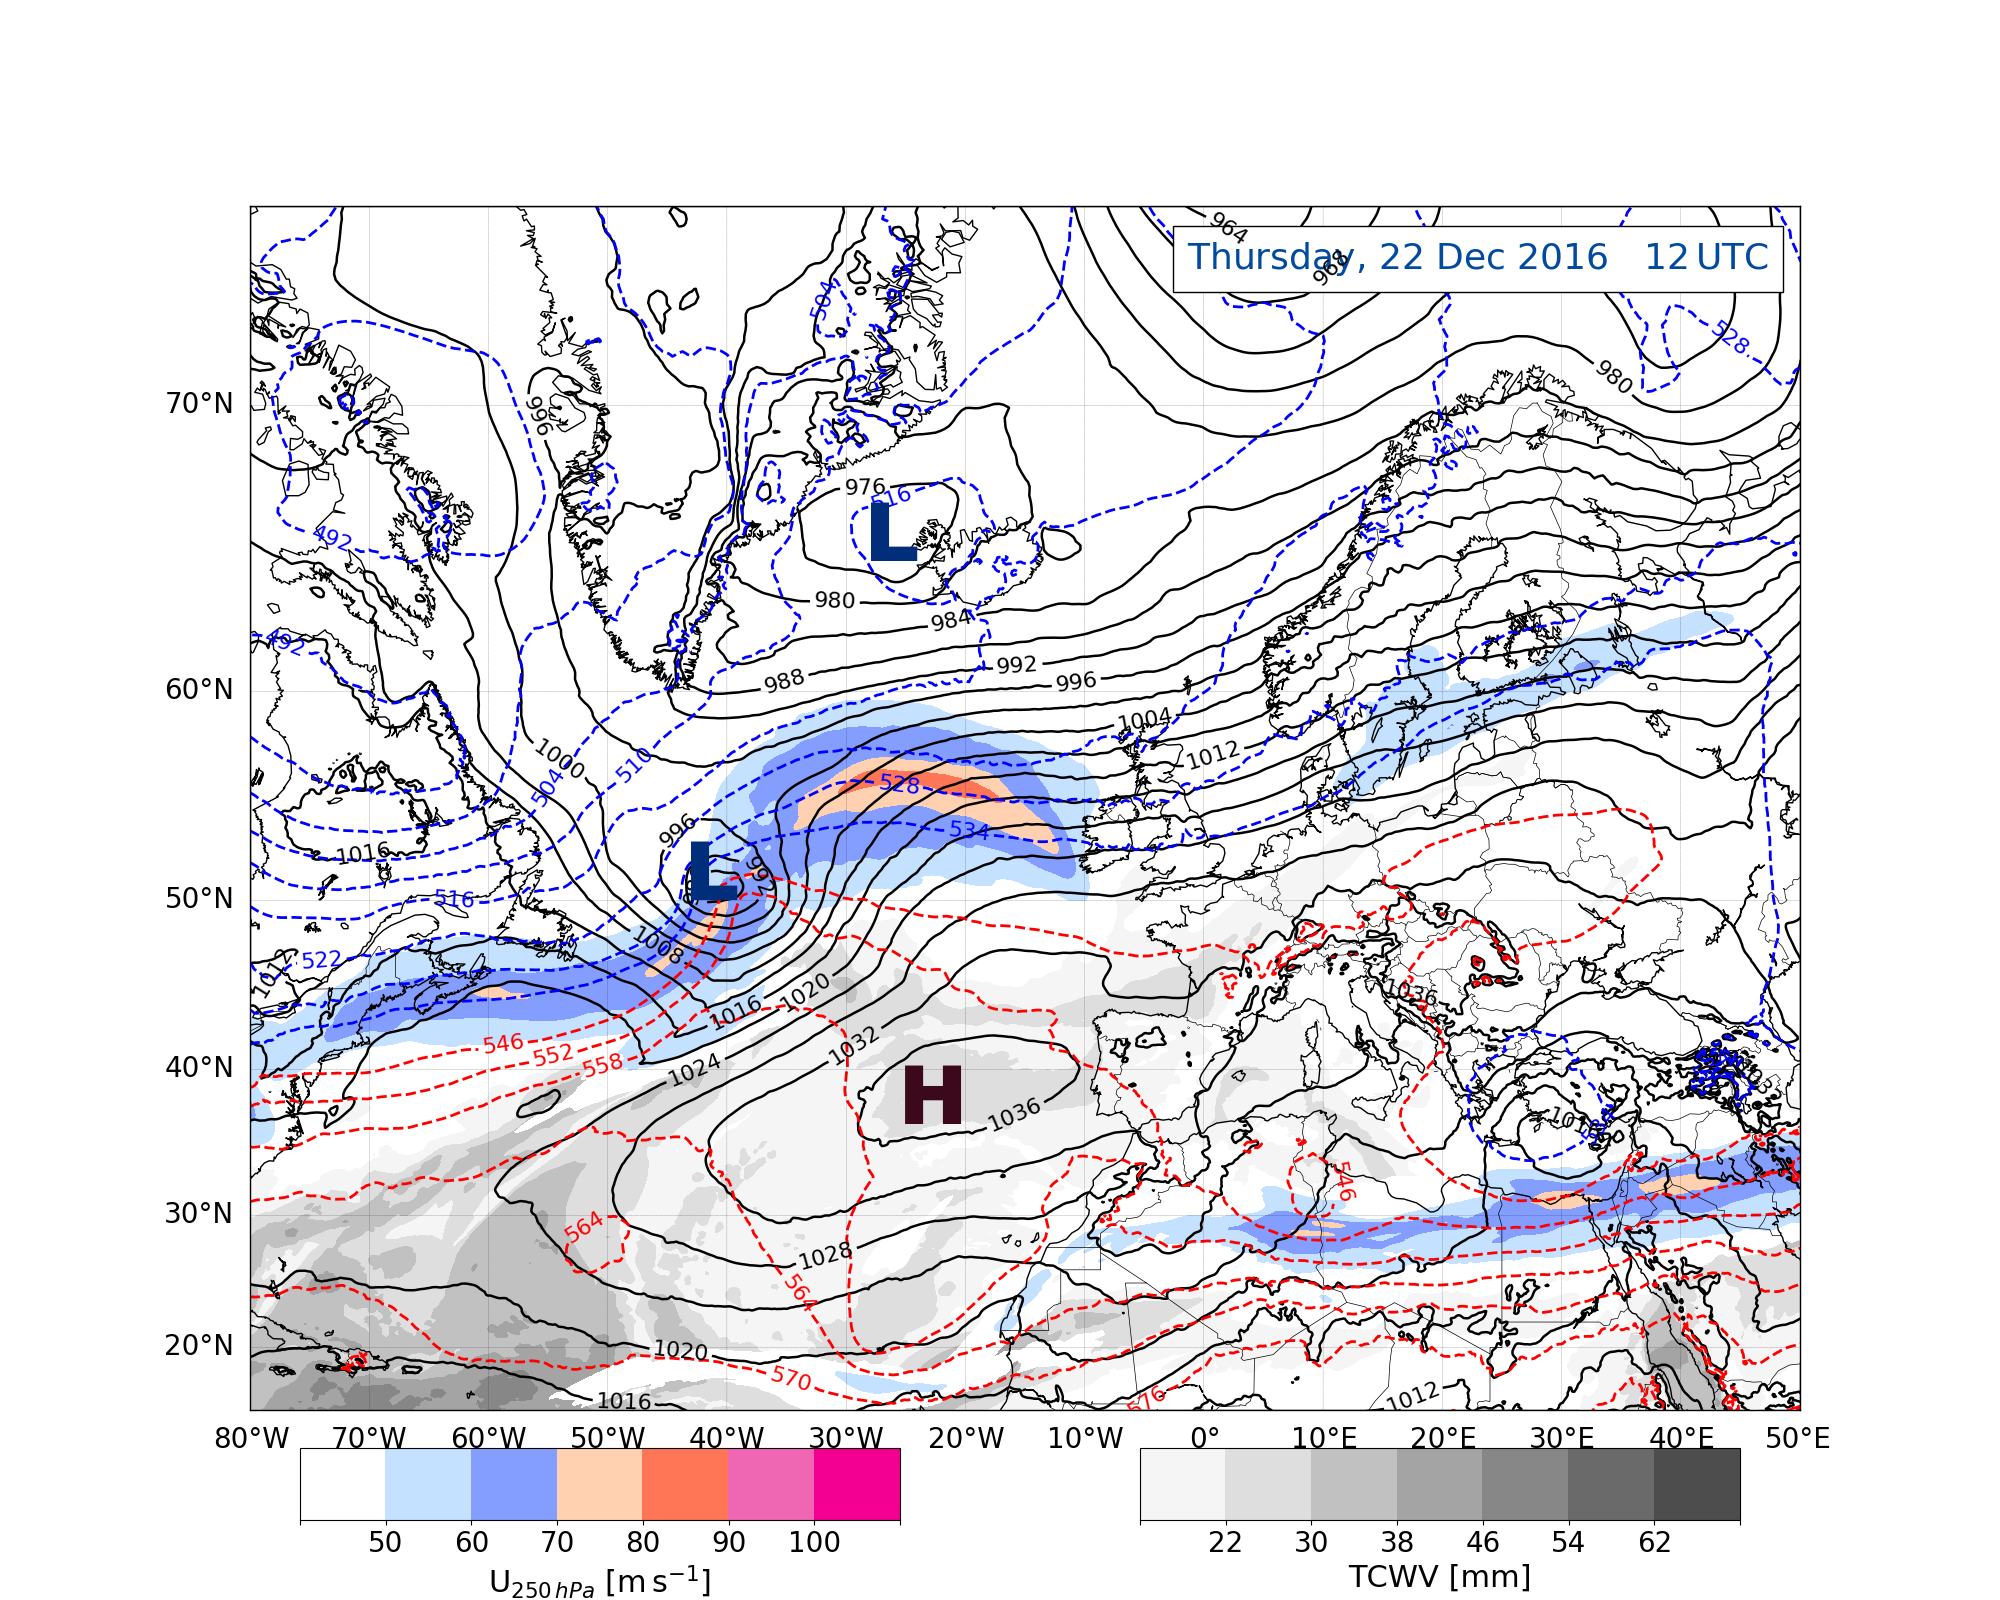
\includegraphics[trim={4.2cm 3.9cm 4.3cm 5.1cm},clip,
	width=\textwidth]{./fig_Geopot_Jet/20161222_12}
		\caption{}\label{fig:GP22}
	%\label{fig:sfc2100}
	\end{subfigure}
%%%%%% 23/12
	\begin{subfigure}[b]{0.49\textwidth}
		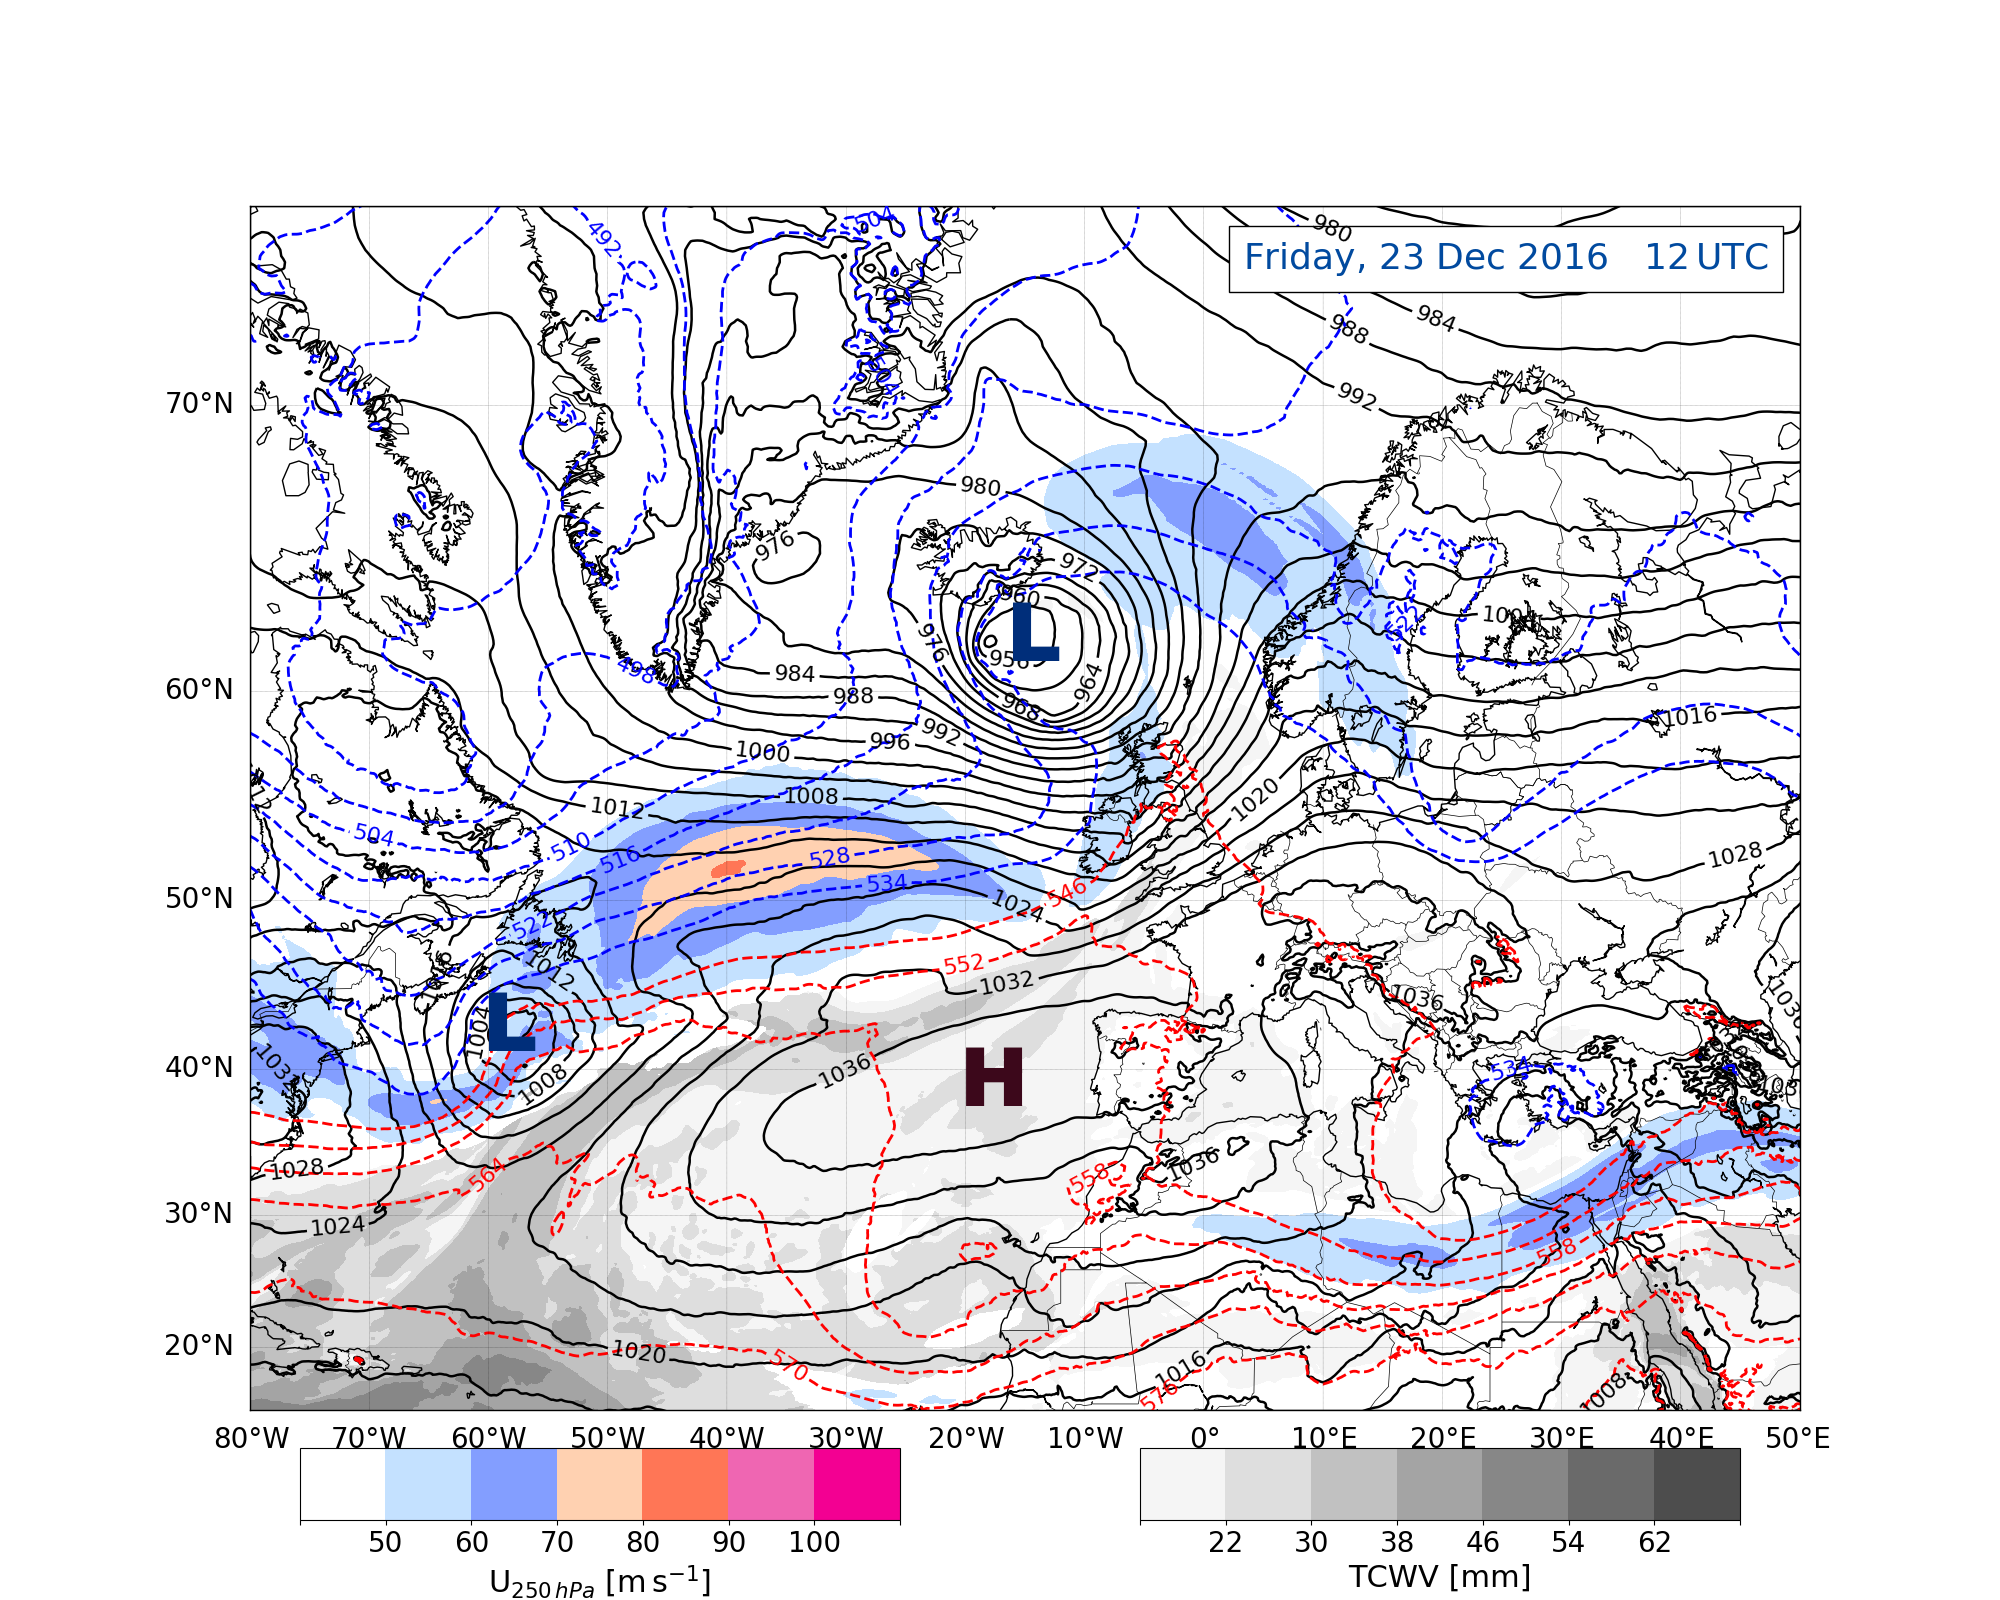
\includegraphics[trim={4.2cm 3.9cm 4.3cm 5.1cm},clip,
	width=\textwidth]{./fig_Geopot_Jet/20161223_12}
		\caption{}\label{fig:GP23}
	\end{subfigure}
%%%%%% label
    \begin{subfigure}[b]{\textwidth}
        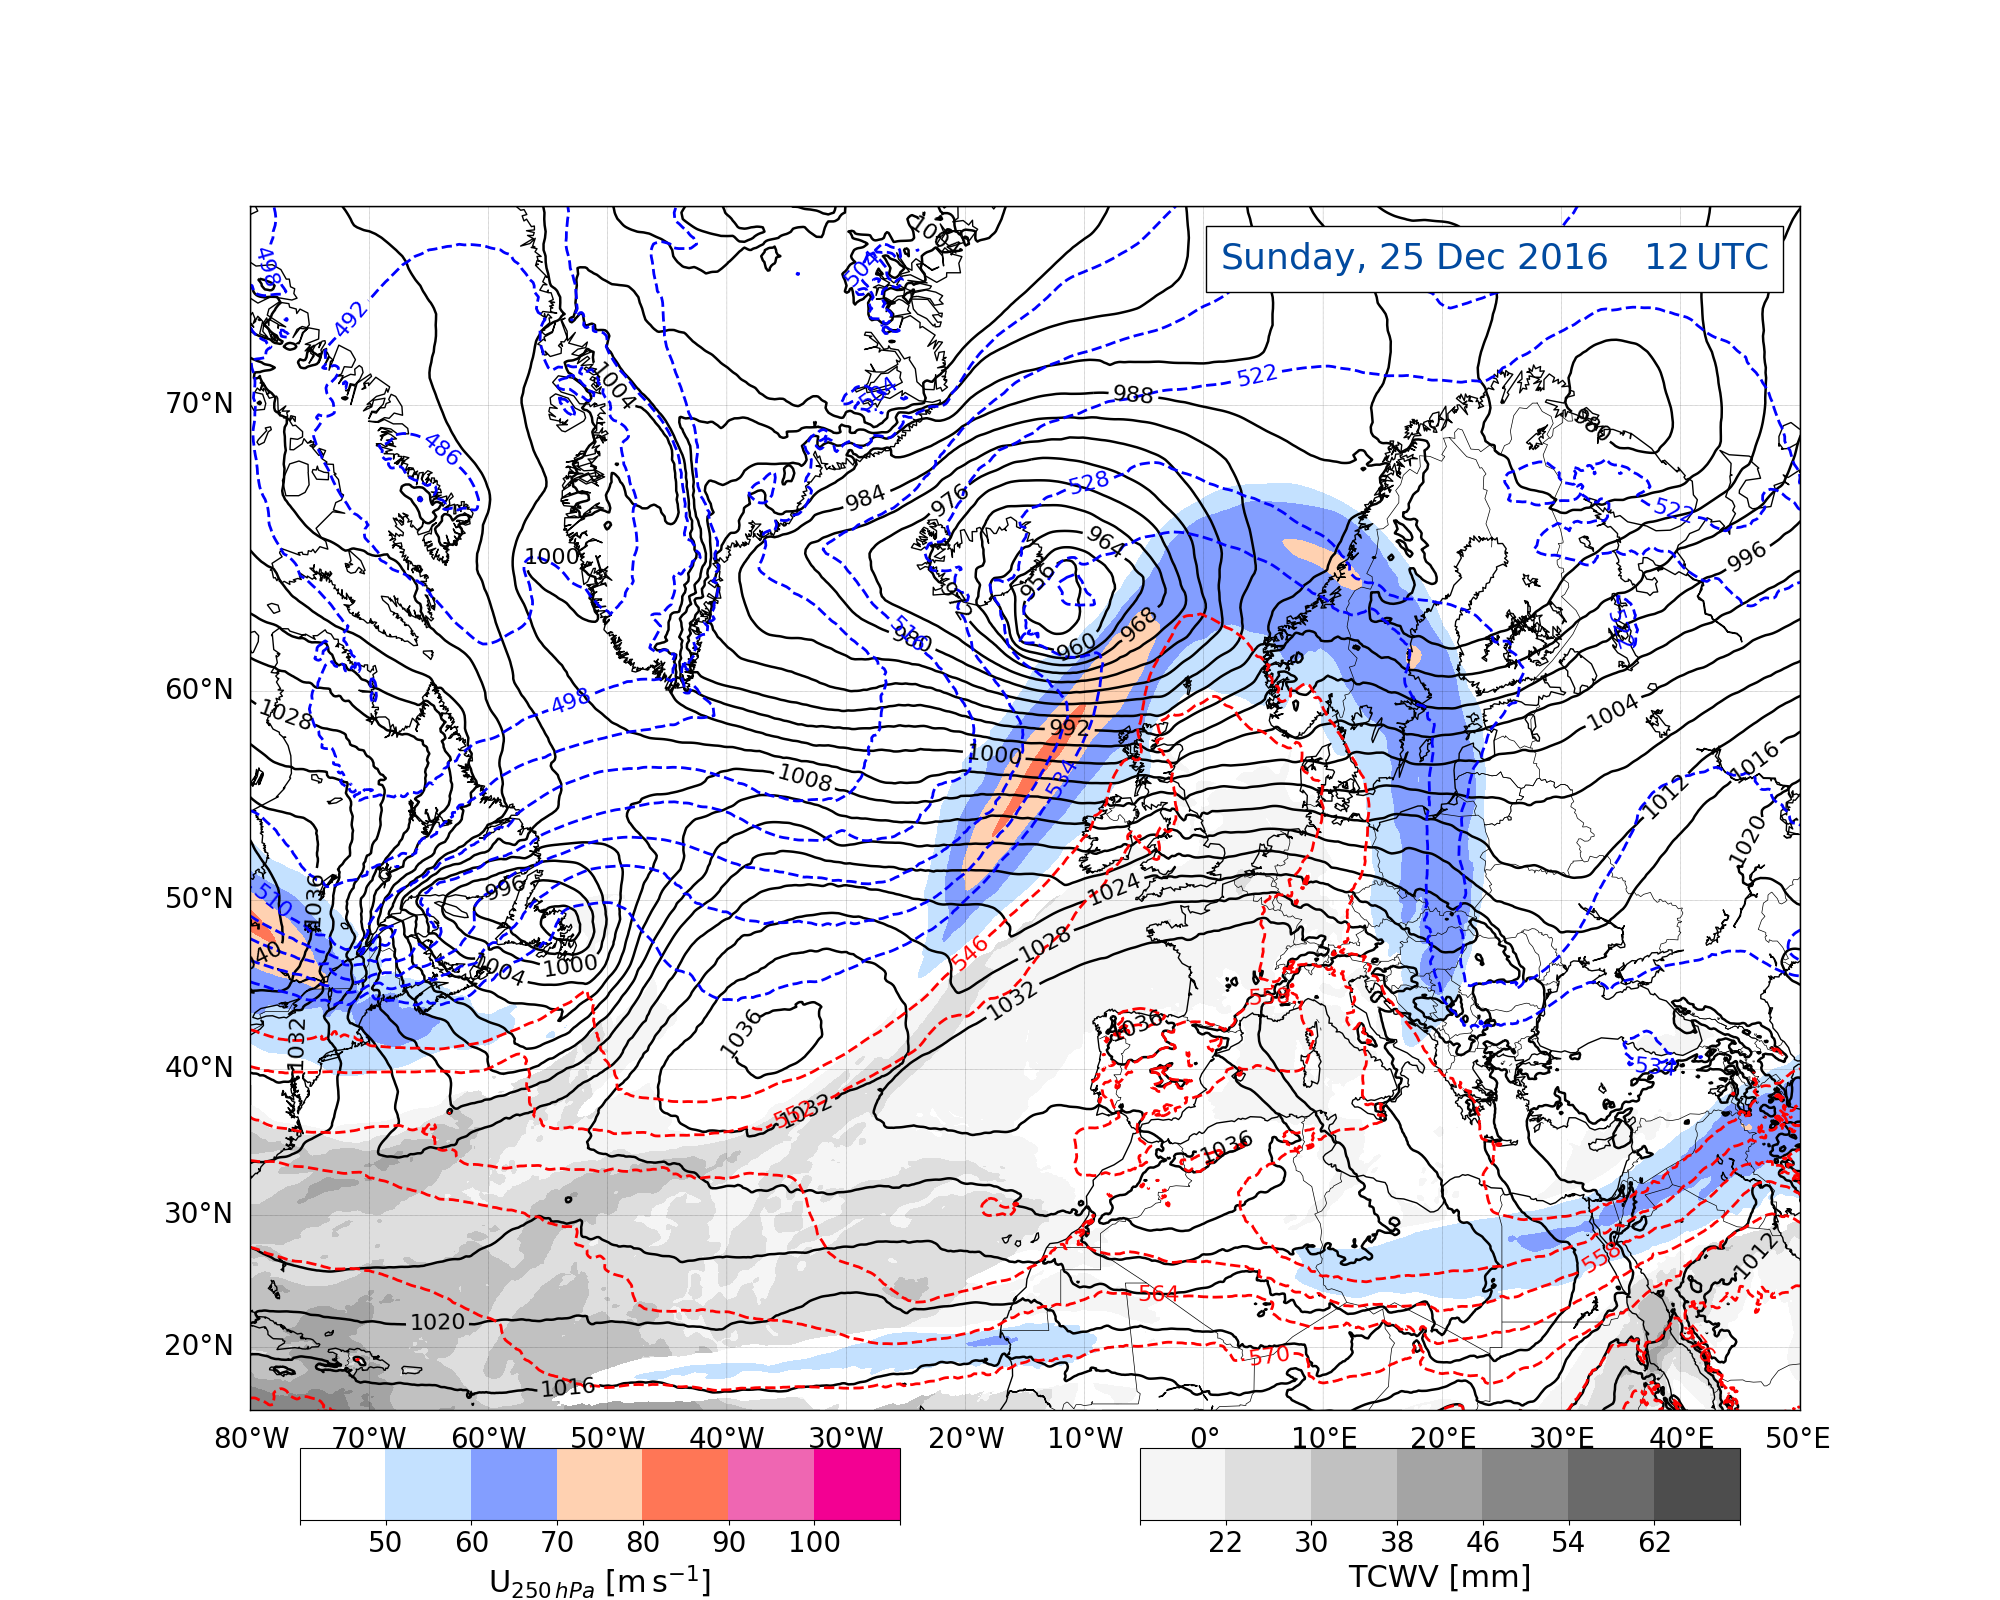
\includegraphics[trim={4.2cm 0cm 4.3cm 36.8cm},clip,
        width=\textwidth]{./fig_Geopot_Jet/20161225_12}
    \end{subfigure}
\caption{Jet, thickness, mean sea level pressure, and moisture synoptic analysis, data from ECMWF. During \SIrange{20}{27}{\dec}. \SI{250}{\hPa} wind speed, shaded according to the colour bar, [\SI{}{\mPs}]. \SI{1000}-\SI{500}{\hPa} thickness, dashed contours every \SI{6}{\deca\meter}, MSLP, black contours every \SI{4}{\hPa}, total column water vapour [\SI{}{\mm}], shaded according the grey scale.}\label{fig:GeopJet}
\end{figure}
\begin{figure}\ContinuedFloat
	\centering
%%%%%% 24/12
    \begin{subfigure}[b]{0.49\textwidth}
        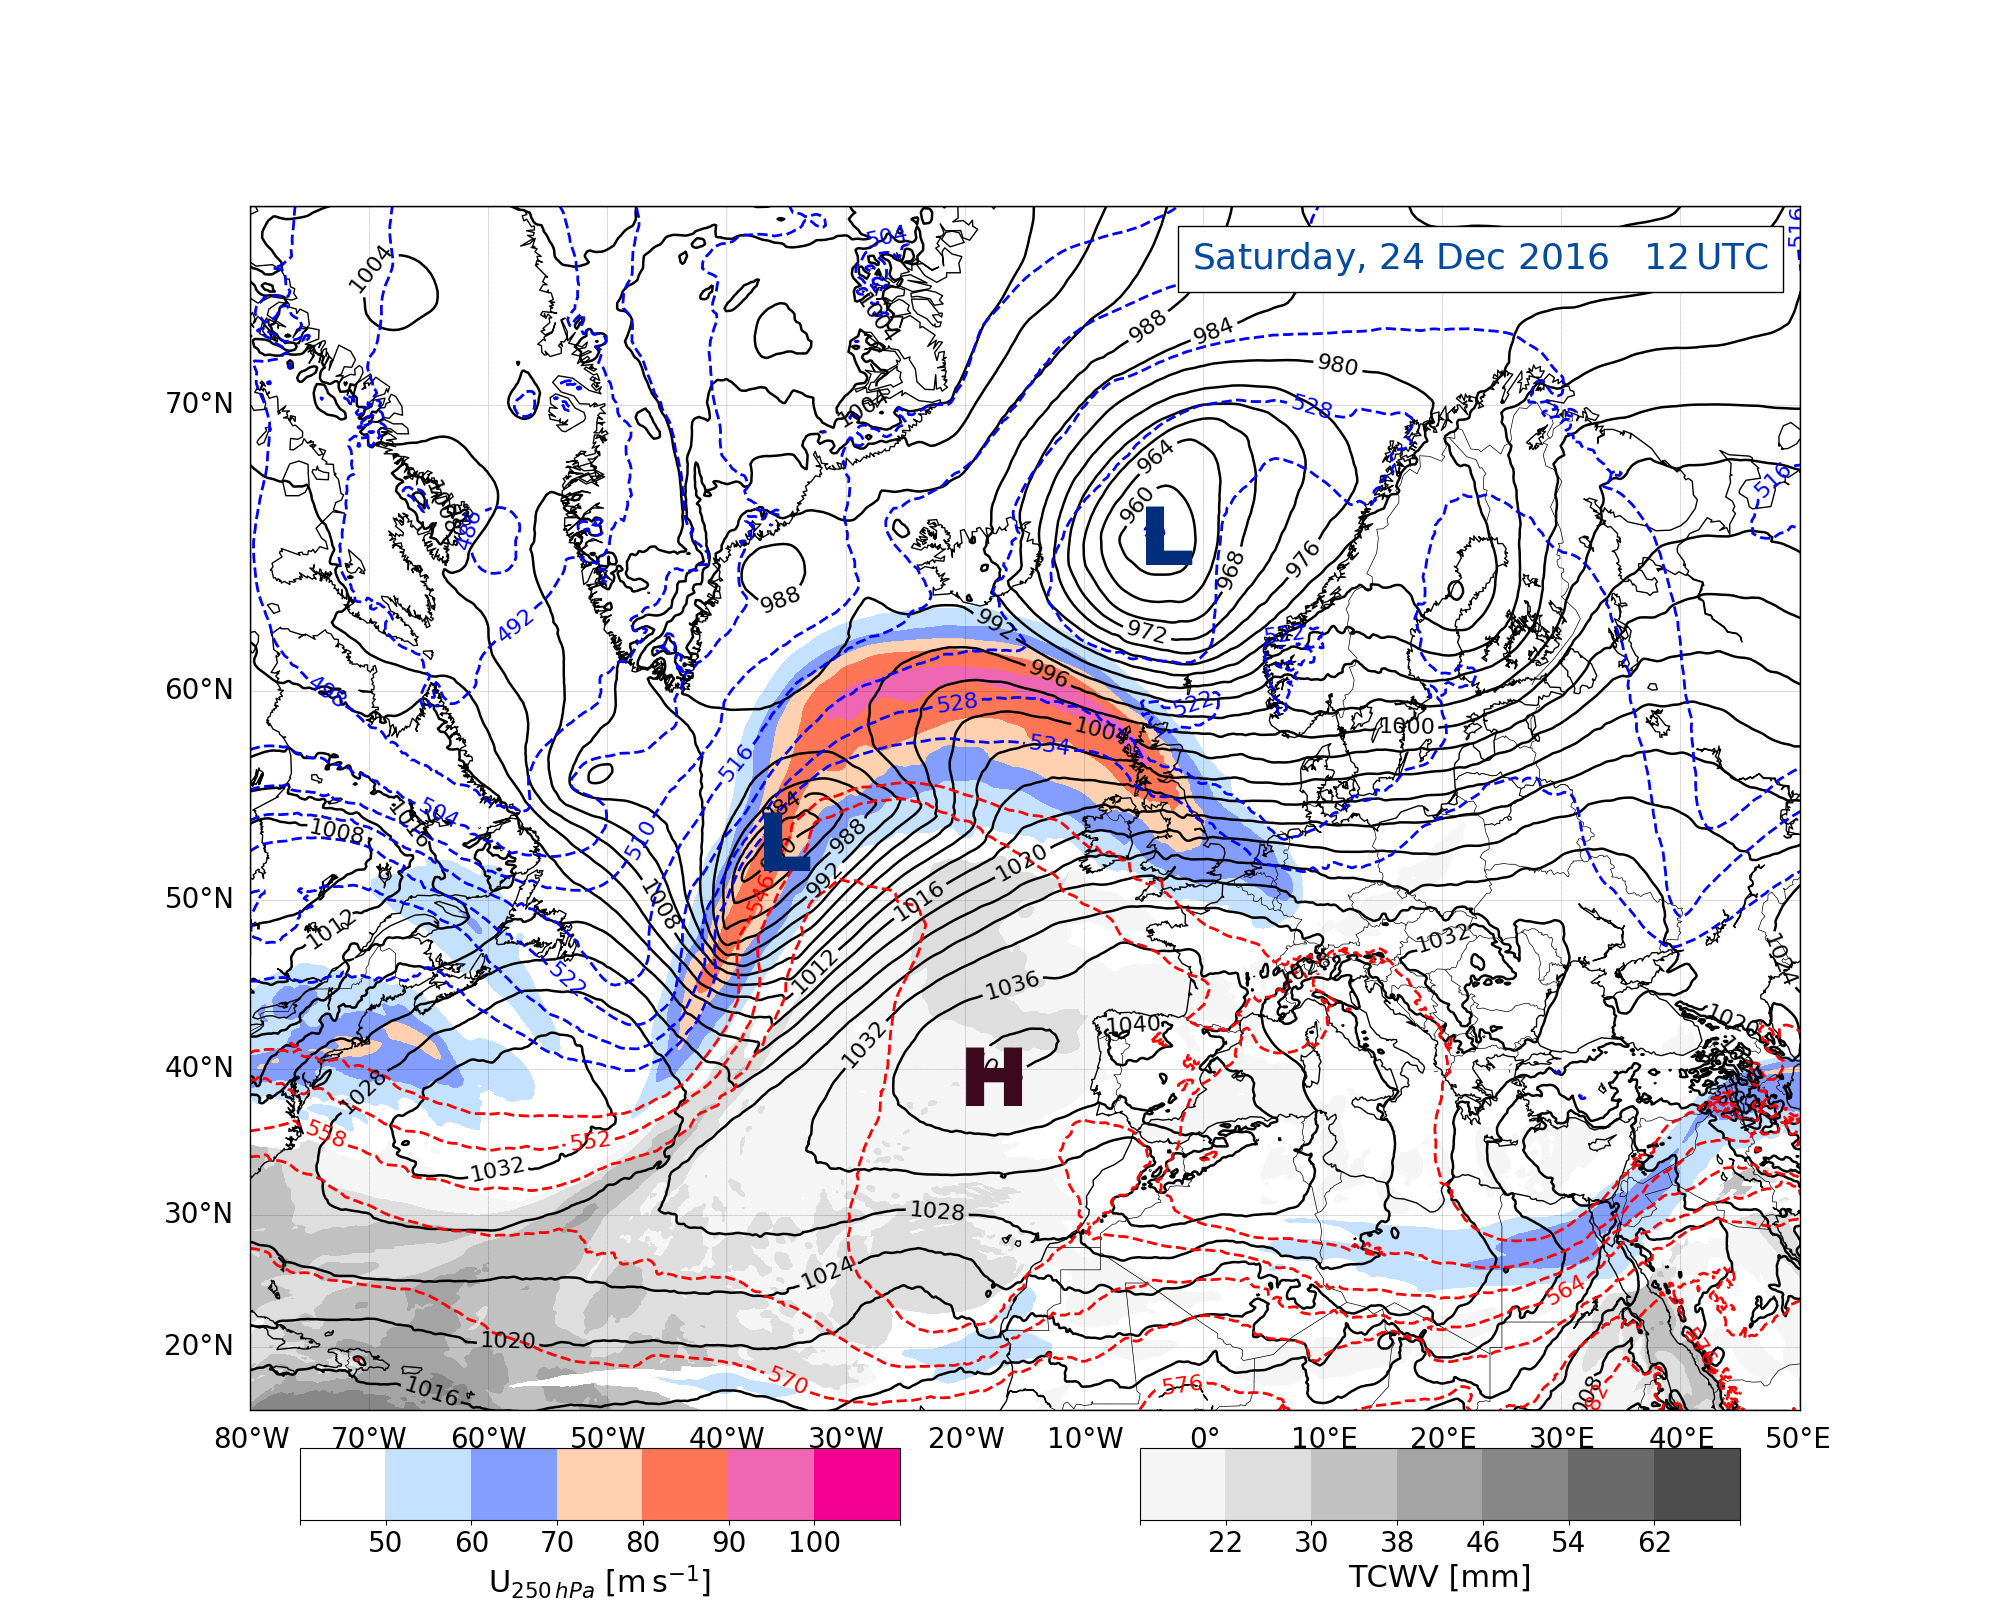
\includegraphics[trim={4.2cm 3.9cm 4.3cm 5.1cm},clip,
        width=\textwidth]{./fig_Geopot_Jet/20161224_12}
        \caption{}\label{fig:GP24}
    \end{subfigure}
%%%%%% 25/12
    \begin{subfigure}[b]{0.49\textwidth}
        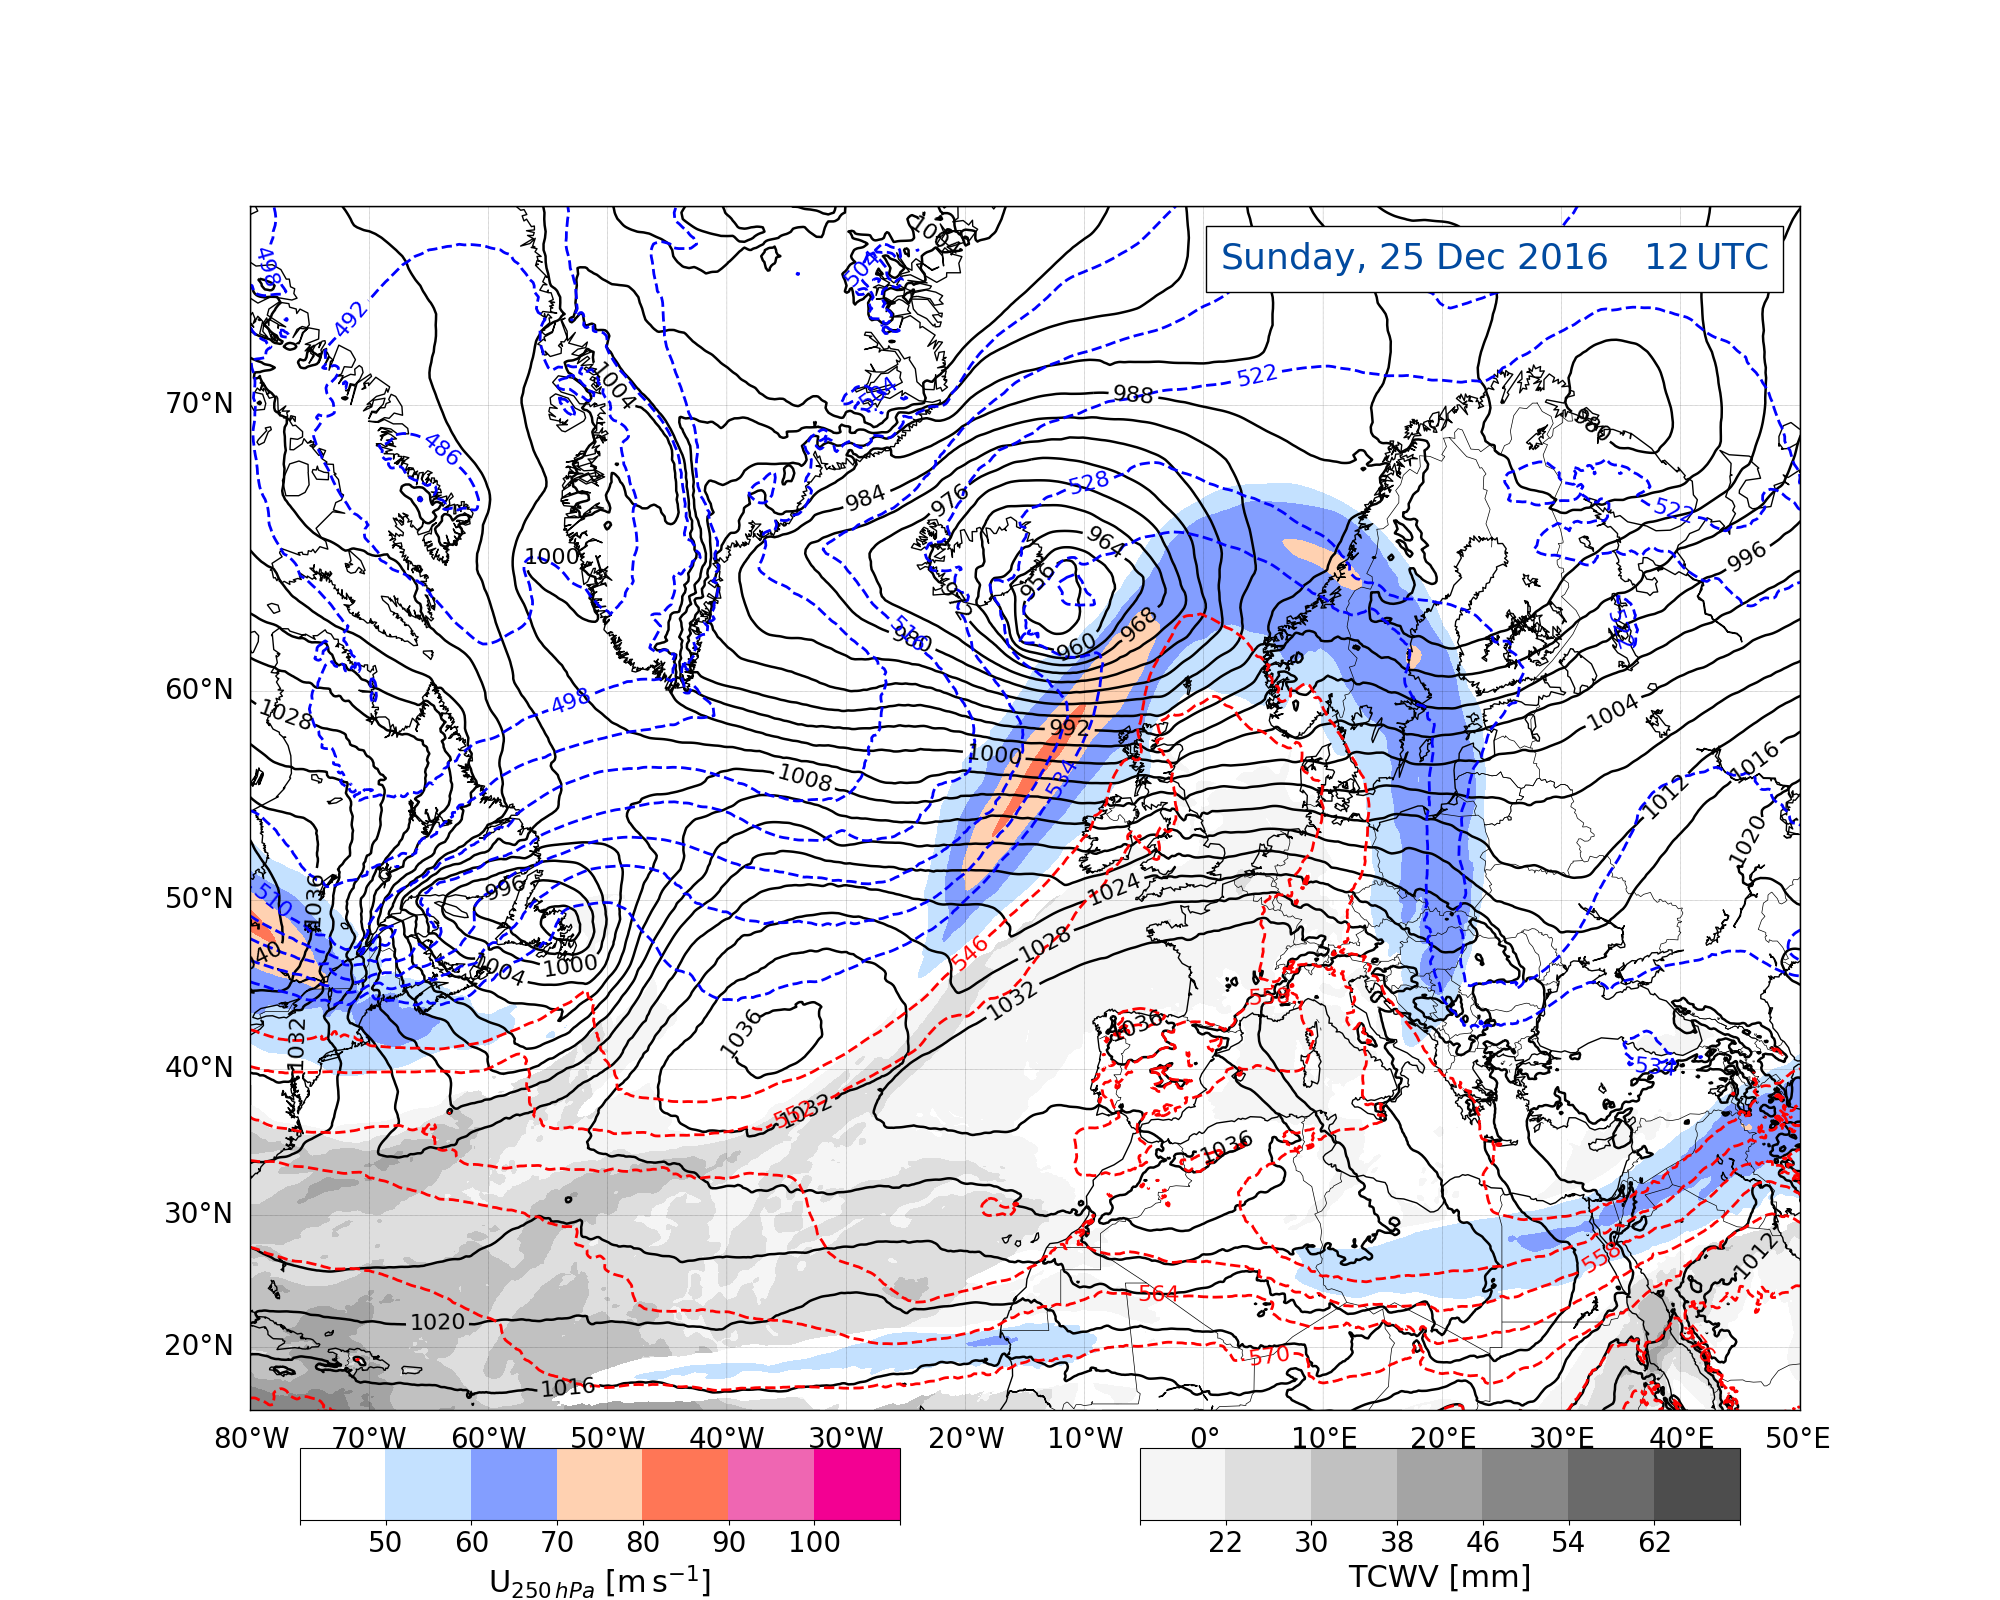
\includegraphics[trim={4.2cm 3.9cm 4.3cm 5.1cm},clip,
        width=\textwidth]{./fig_Geopot_Jet/20161225_12}
        \caption{}\label{fig:GP25}
    \end{subfigure}
%	\centering
%%%%%% 26/12
    \begin{subfigure}[b]{0.49\textwidth}
        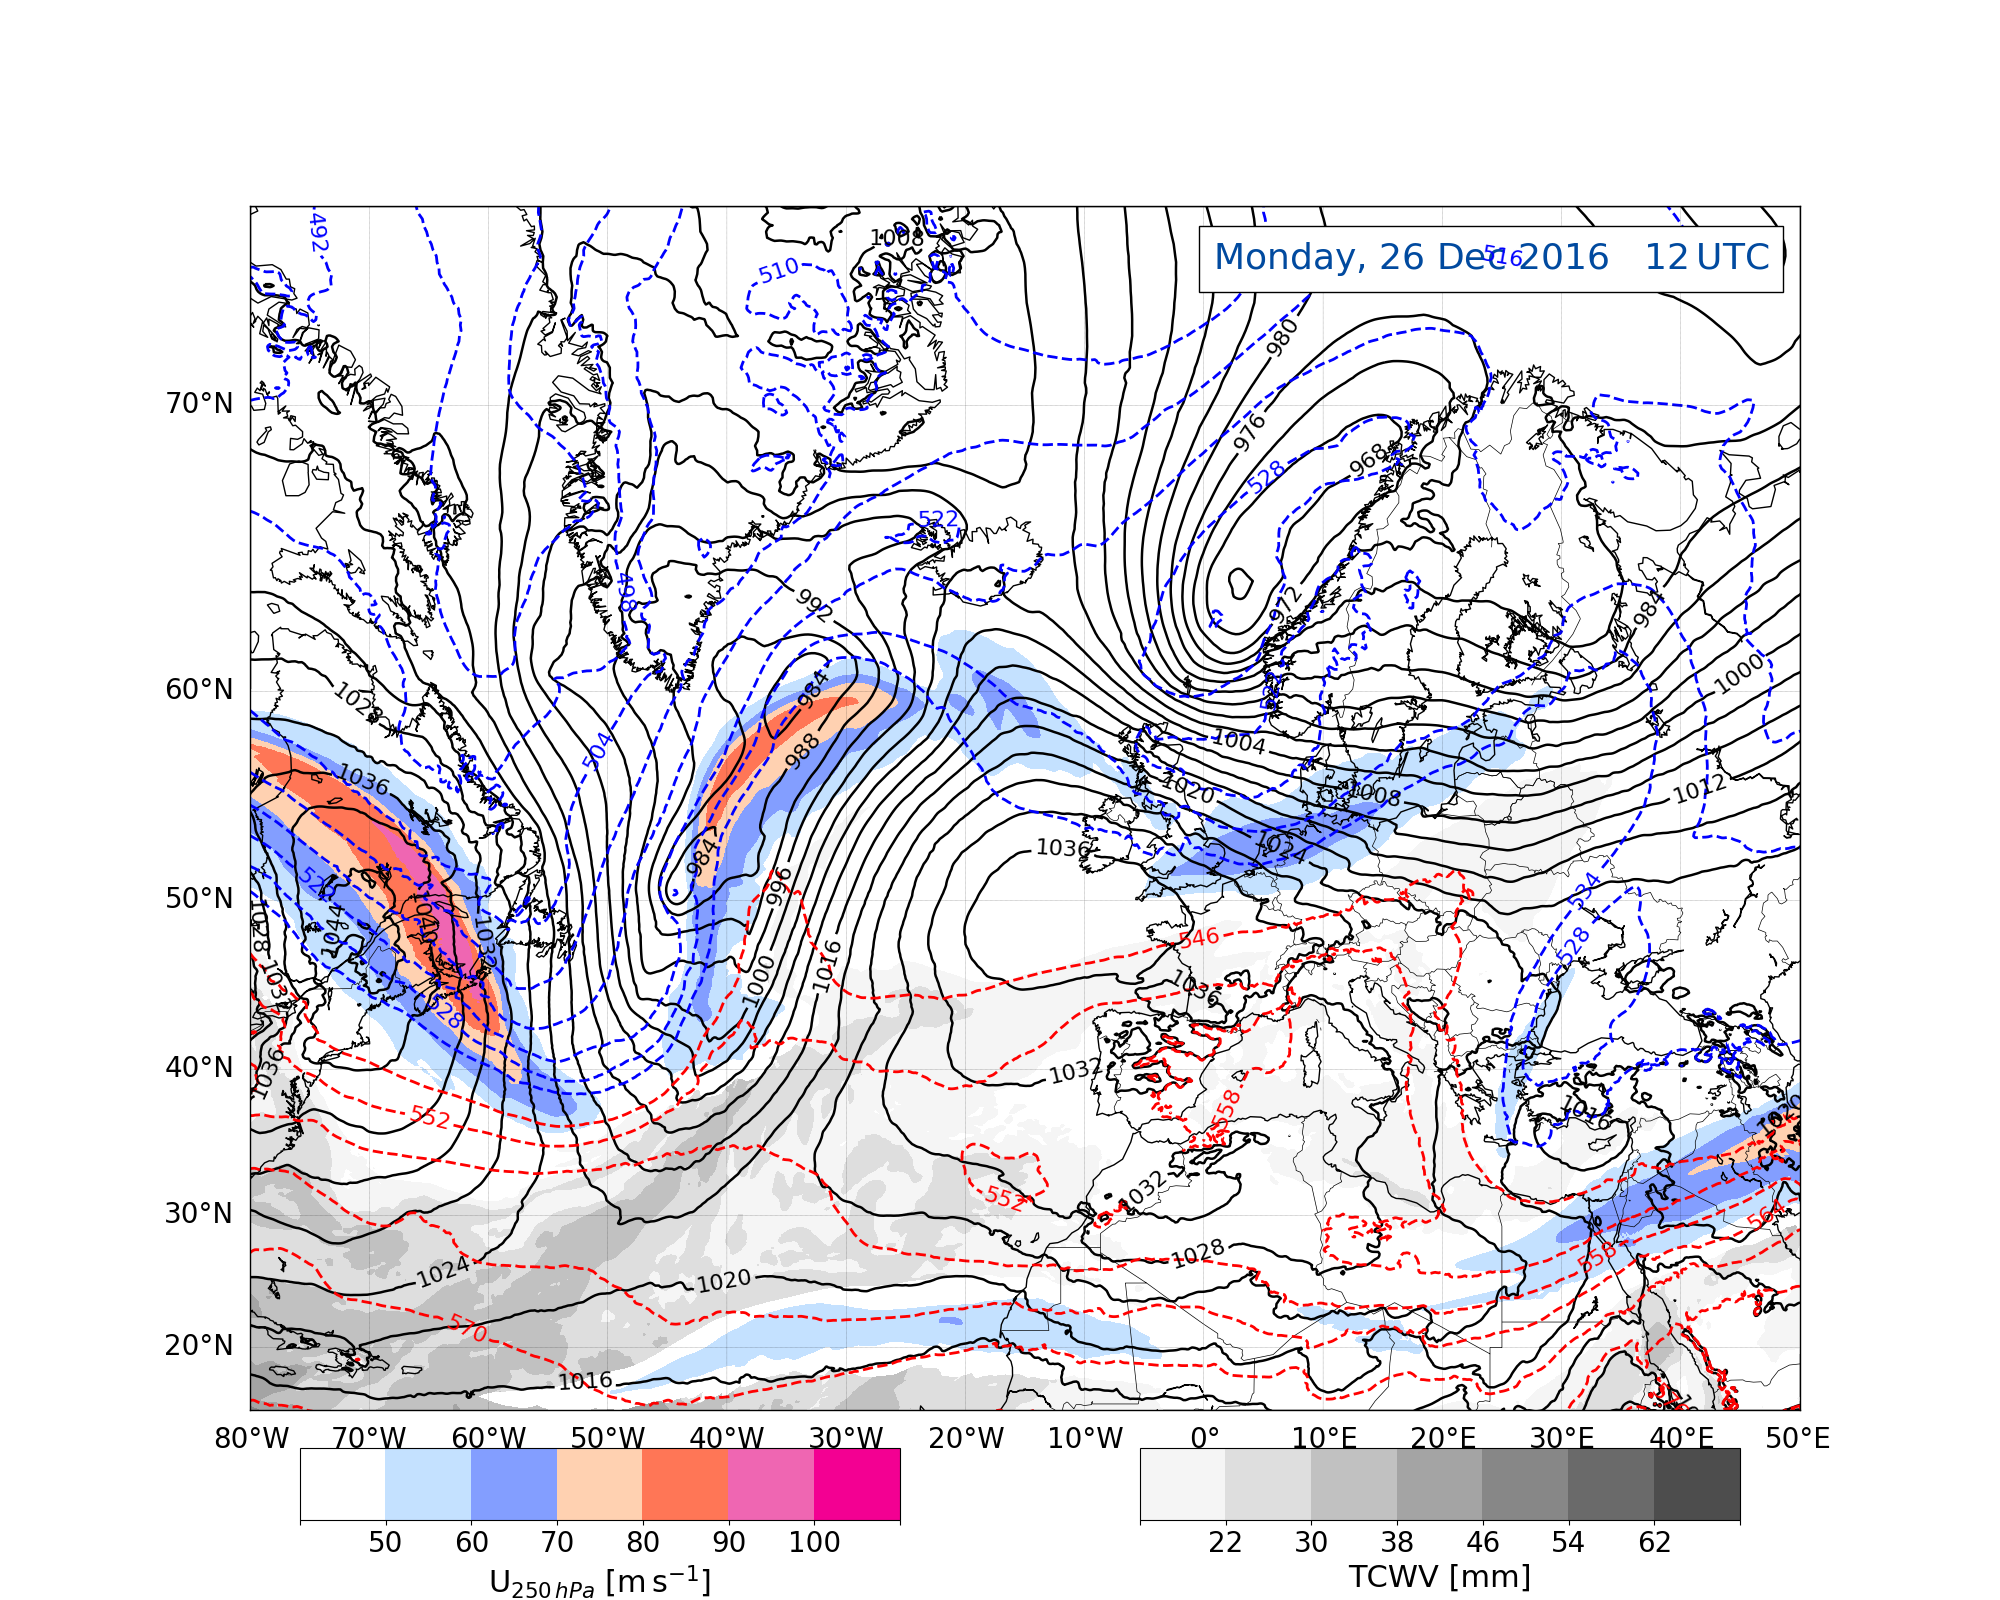
\includegraphics[trim={4.2cm 3.9cm 4.3cm 5.1cm},clip,
        width=\textwidth]{./fig_Geopot_Jet/20161226_12}
        \caption{}\label{fig:GP26}
    \end{subfigure}
%%%%%% 27/12
    \begin{subfigure}[b]{0.49\textwidth}
        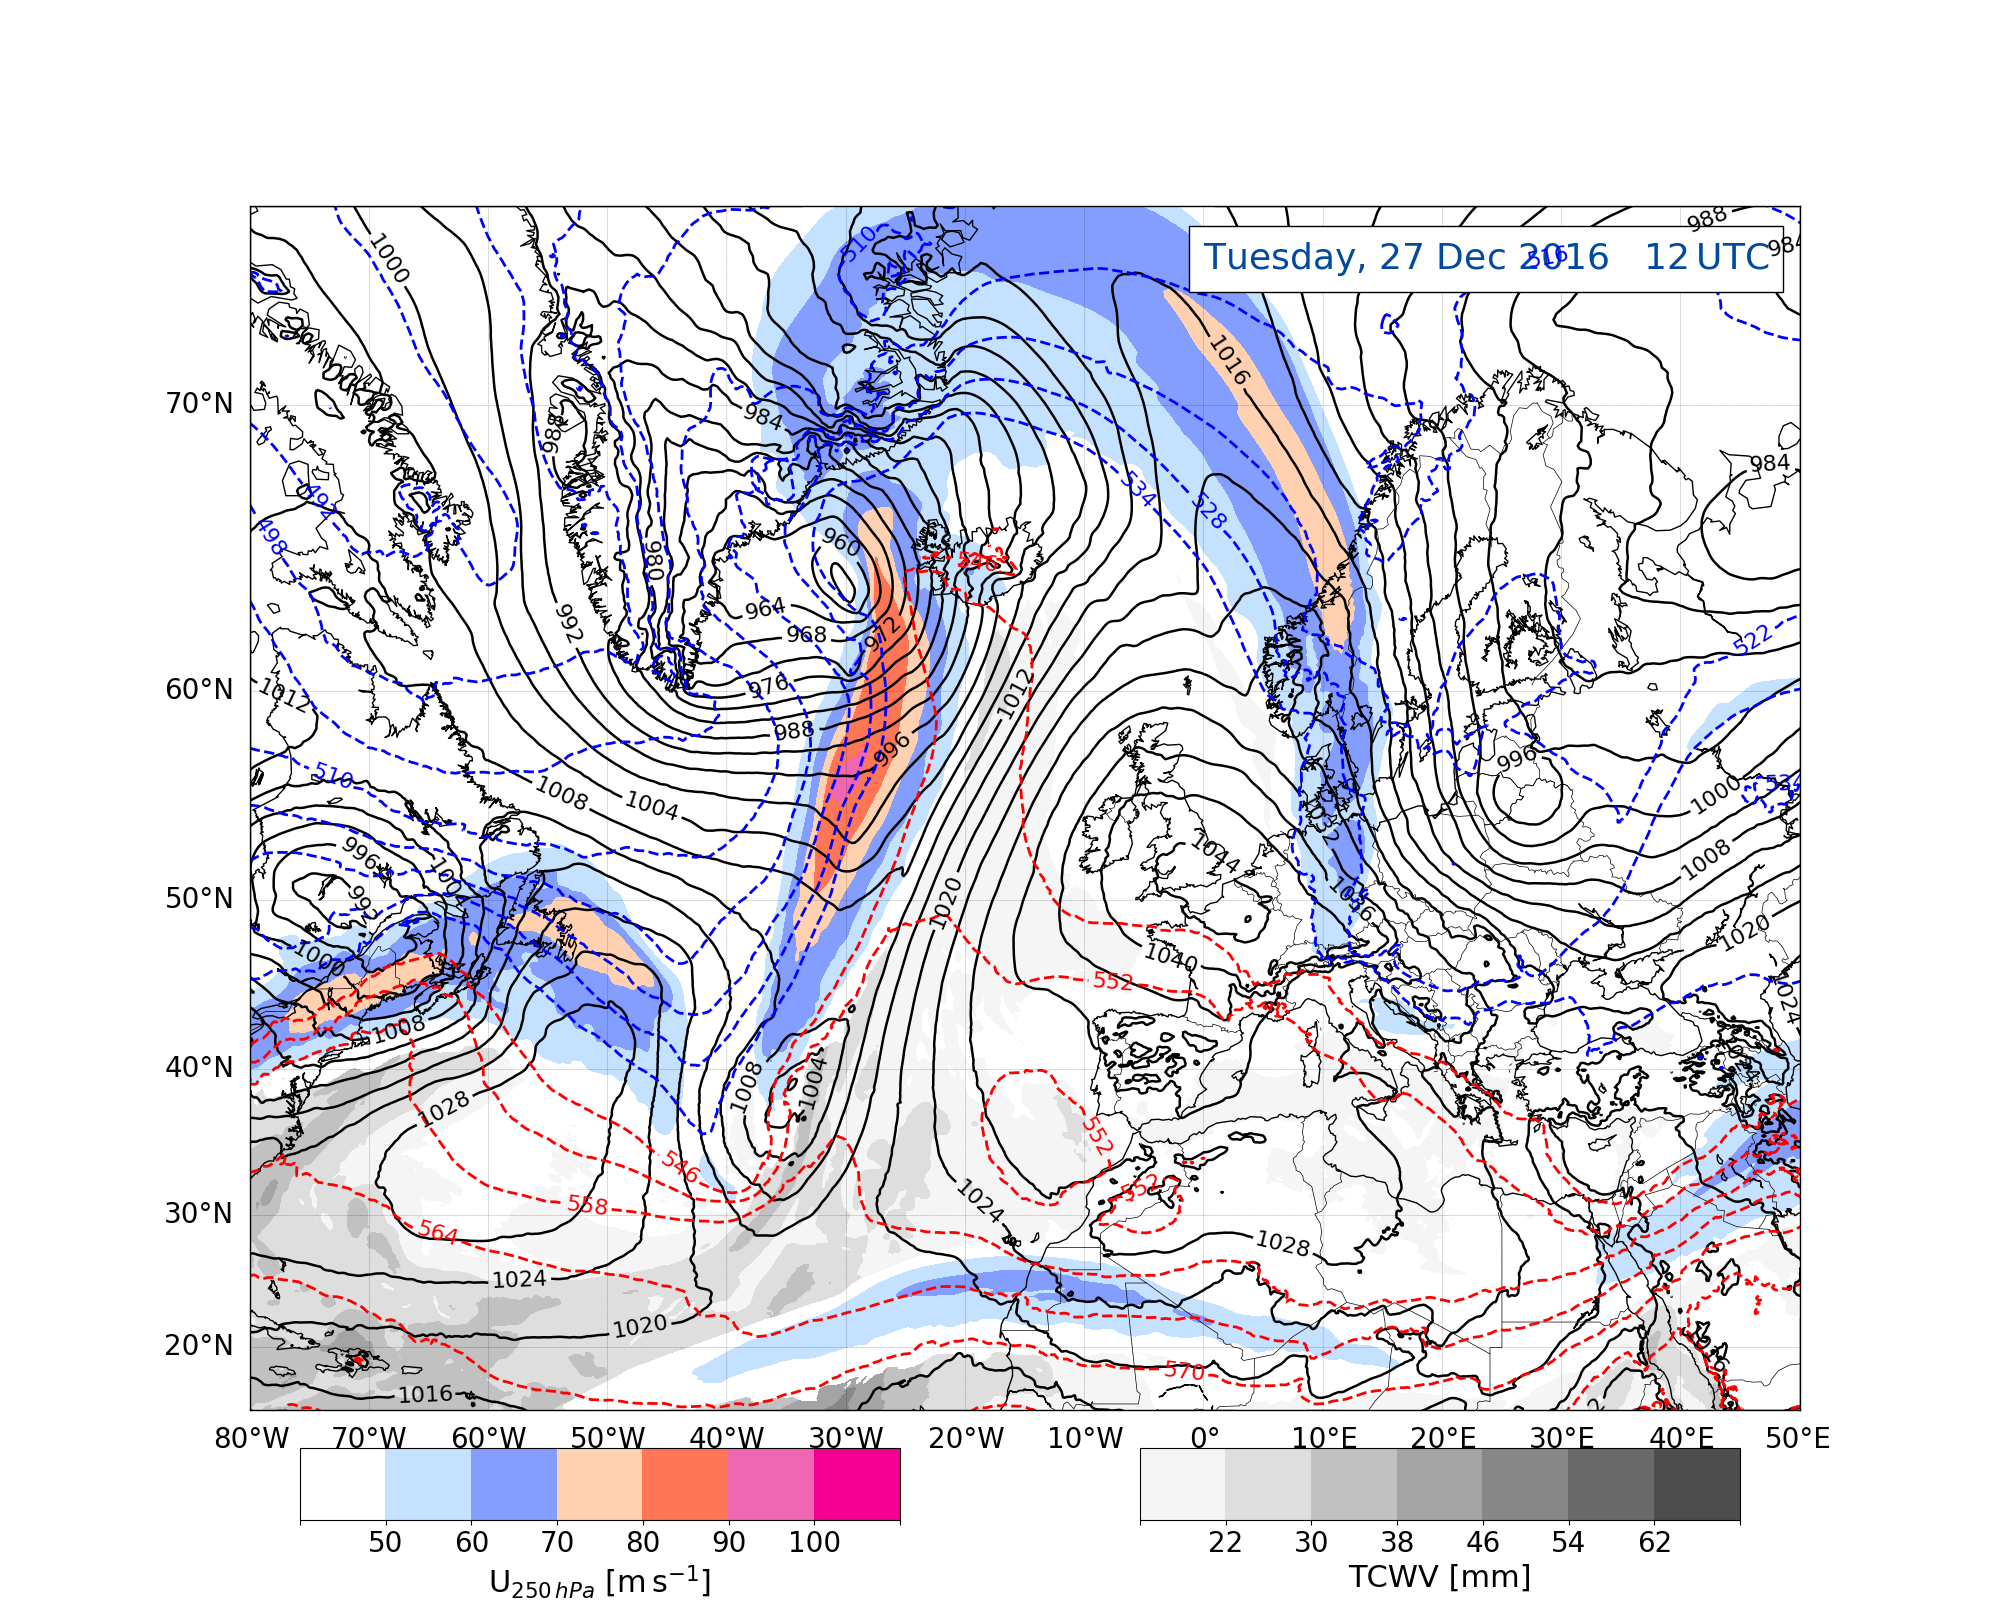
\includegraphics[trim={4.2cm 3.9cm 4.3cm 5.1cm},clip,
        width=\textwidth]{./fig_Geopot_Jet/20161227_12}
        \caption{}\label{fig:GP27}
    \end{subfigure}
%%%%%% label
    \begin{subfigure}[b]{\textwidth}
        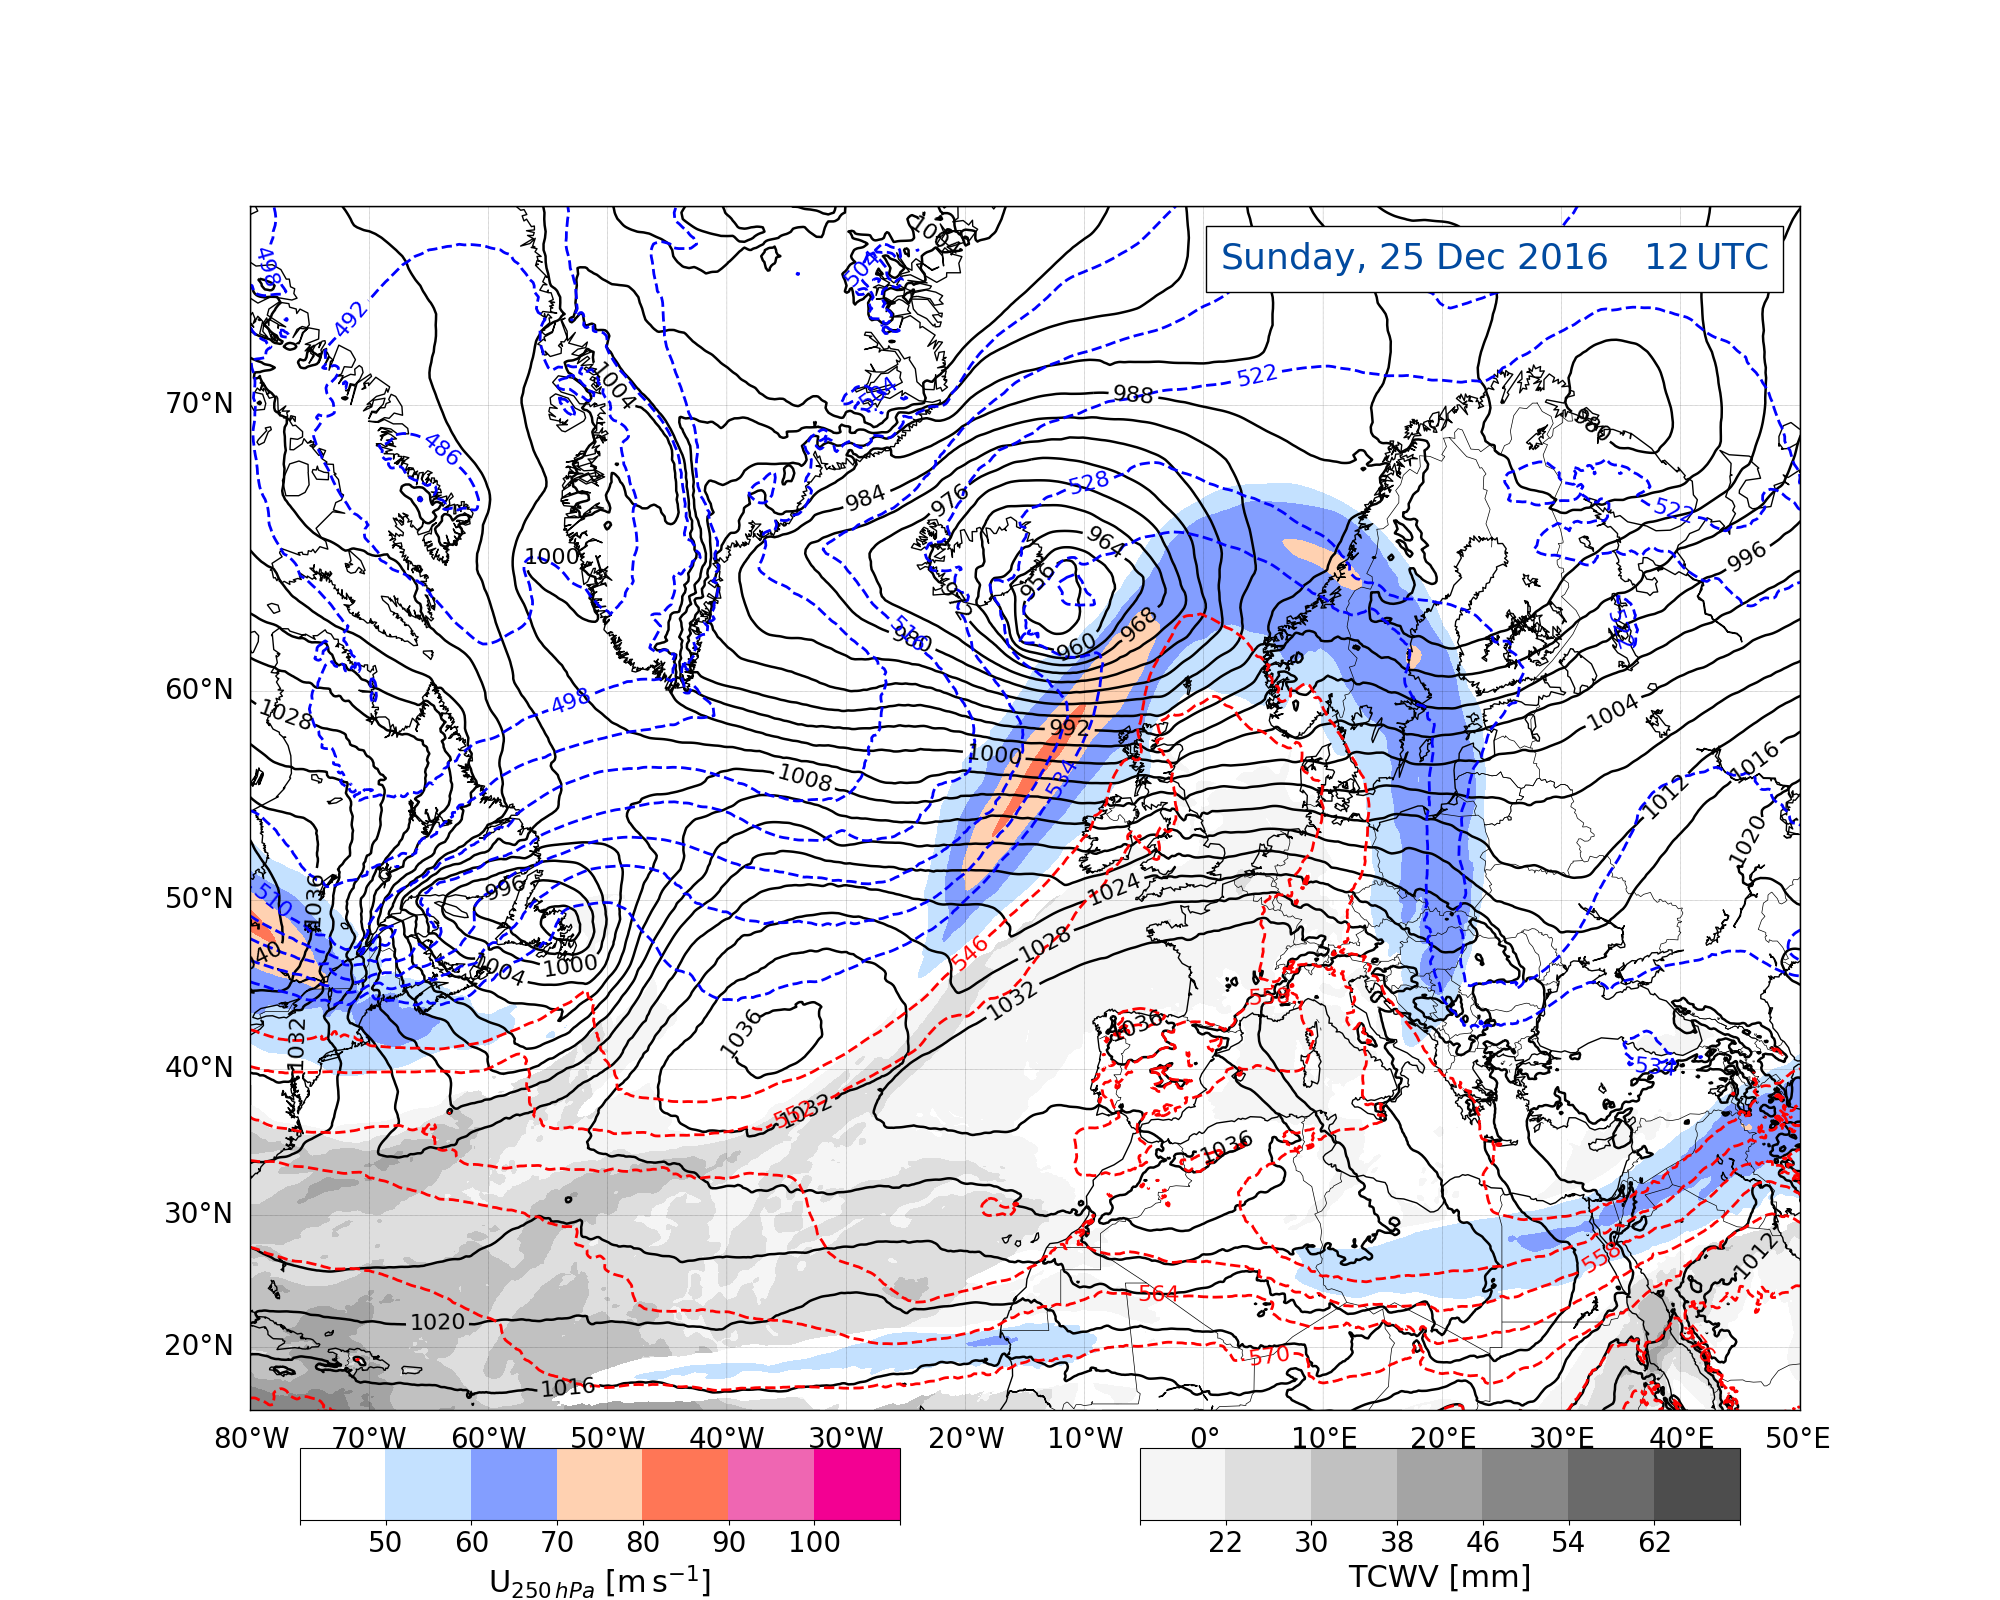
\includegraphics[trim={4.2cm 0cm 4.3cm 36.8cm},clip,
        width=\textwidth]{./fig_Geopot_Jet/20161225_12}
       % \label{fig:D}
    \end{subfigure}
\caption{\textit{(Continued from previous page.)}}   
\end{figure}